As this project is focused on the resource management framework, I will
not give a detailed description of the Hadoop Distributed File
System. Yet, I will go through some basic concepts that will make the
reader understand better the overall architecture of Hadoop.

HDFS is the distributed file system of Hadoop platform. It is designed
with the assumption that hardware failure is the norm and not an
exception making it highly fault-tolerant. Also, it is designed to run
on commodity, heterogeneous, low-cost hardware making the setup and provisioning of
a cluster cheaper than in HPC. HDFS has two main entities, the NameNode
(NN) and the DataNode (DN) and its architecture is depicted in Figure
\ref{fig:hadoop_hdfs}.

\begin{figure}
\centering
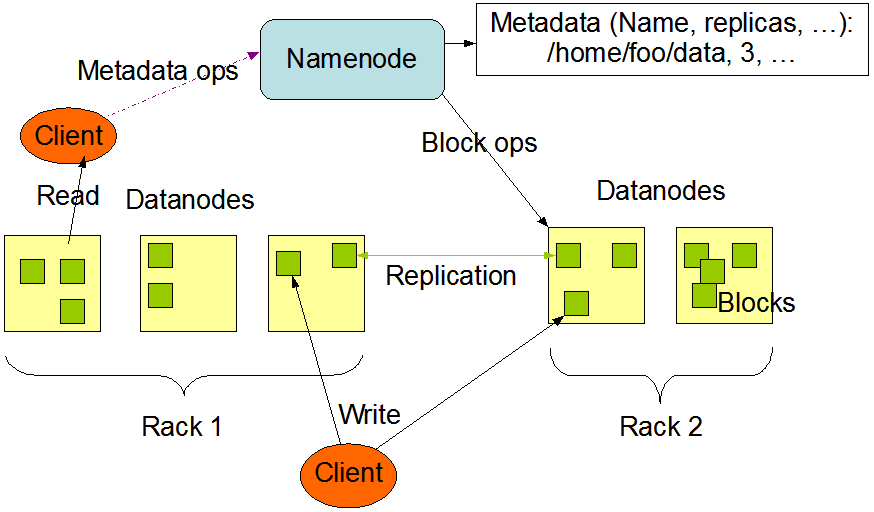
\includegraphics[scale=0.5]{resources/images/Background/hdfs_arch.png}
\label{fig:hadoop_hdfs}
\caption{HDFS architecture \cite{hdfs}}
\end{figure}

\subsection{NameNode}
\label{ssec:nn}

An HDFS cluster consists of a single active NN that is responsible for the
file system metadata, the blocks replication and the health
status of the DNs.

HDFS exposes to a user a file system similar to POSIX, in terms that
the structure is hierarchical, there are the same file permissions 
and a subset of POSIX operations. A user through the NN can open,
close, read, delete a file as in any file system. The NN uses a transaction
log, the \emph{EditLog}, that persists to the local file system any
operation that is done to the HDFS namespace. For example if a file is
renamed then a record is added to the EditLog, or if the replication
factor for a file is changed.

As HDFS was designed to run on commodity
hardware it should be able to handle machine failures. Internally, a
file is split in a number of blocks. Typically each block is 128 MB,
except from the last one and are stored
in the DNs. HDFS replicates the blocks to other machines--DNs
according to a configurable replication factor and replication policy.
If the DN that holds a specific block has crashed, then that block is read from
another replica in another DN.
The NN keeps a file in its local file system with the entire namespace
and the mapping of blocks to DNs, called \emph{FsImage}. Upon
recovery, the NN reads the FsImage and applies any operation that is
logged in the EditLog. That way it can recover from a scheduled
maintenance reboot or from a crash.

The NN periodically receives heartbeats from the DNs that have dual
purpose. The first one is to maintain a health status for the DNs. If
the NN misses a heartbeat from a DN, then it marks that DN as
dead. From that point no blocks will be further assigned to that DN
and NN will start migrating all the blocks that reside in that DN to
others. The second reason of receiving heartbeats is to maintain an
updated view of the \emph{BlockMap}, the mapping of blocks to
DNs. When a DN sends a heartbeat to the NN, it piggybacks a list with
the blocks that it currently stores. That way, the BlockMap in the NN
is kept up-to-date with the blocks that are stored in every DN.

\subsection{DataNode}
\label{ssec:dn}

The DN is the slave entity in the HDFS master/slave architecture as depicted in
Figure \ref{fig:hadoop_hdfs} and the actual storage of blocks. Upon a
client request to store a file in HDFS, the NN instructs it (the
client) which DNs to contact to store the individual file block. The
same procedure is followed when a client requests to read a file. The
NN returns a list with DNs that store the blocks forming the whole
file. The client then contacts each and every DN, fetching the
corresponding blocks.

A DN periodically heartbeats to NN. As I have explained in Section
\ref{ssec:nn}, the heartbeat contains a list of blocks, that the DN
issued the heartbeat stores, so that the NN maintains a map of file
blocks and DataNodes. Also, the heartbeat signifies that the DN is
alive and can be used for storage and retrieval of blocks. Heartbeats
also carry information regarding the status of the DN such as total
storage capacity, storage in use etc. These metrics are taken
consideration by the NN when assigning blocks to DN.

The DataNode also perform various operations as instructed by the
NN. These instructions are sent to the DN via the heartbeat
mechanism as a reply to the heartbeat sent by the DN. Such operations
might be creation, deletion or replication of a block. The block
replication is done according to the replication strategy. A common
strategy for placing replicas with a replication factor of three, is
to place the first replica in the same node as the client runs, the
second in another node in a different rack (off-rack) and the third
one in the same rack as the second but in a different node. Adjusting
the replication factor and the replication policy can greatly affect
the write and read performance of the HDFS cluster and should be
carefully tweaked.
